\chapter{Na-22 measurement}

% perche misurare a questa energia e come

\section{Phenomenology}

The physics of $\gamma$ photon interaction have been already introduced in chapter 2.
In order to build a time correlated single photon counting experiment two time signals are necessary, a start signal and a stop signal.
A simple way to obtain this is to use a $\beta ^{+}$ active isotope, such as $Na^{22}$. This isotope emits a positron according to the decay reaction $^{22}Na \rightarrow ^{22}Ne + \beta ^{+} + \ni _{e} + \gamma$. The positron yield is relatively high, $90.4\%$, and competitive processes are electron capture (EC) and direct transition to the Ne ground state. 
In the positron emission case the Ne ground state is reached after 3.7 ps by emission of a $\gamma$ quantum of 1.274 MeV. The half life of the isotope is 2.6 years.
\begin{figure}[htbp]
\begin{center}
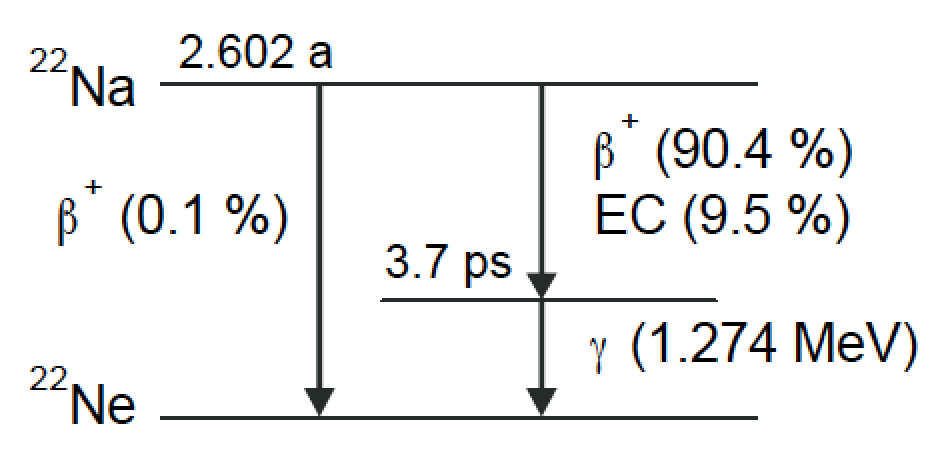
\includegraphics[width=8cm]{../Pictures/Chapter_7/Na-22}
\end{center}
\caption[Na$^{22}$ decay scheme]{Decay scheme of Na$^{22}$}
\label{fig:Na_22}
\end{figure}
It is worth to note that, as outlined in chapter 2 the Cerenkov threshold for heavy scintillators is below the energy of the annihilation gamma produced by the isotope.

% tabella con soglia

\section{Experimental setup}
The components of the apparatus were placed in a cooled black box.
Cooling is necessary to mantain the performance of SiPM
%spiegare perche temperatura stabile

%disegnino
The start signal is obtained by mean of a LSO crystal. The reference crystal is readout by a SiPM board amplified by a NINO chip. 
%spiegare e mostrare il setup della board

%stop signal is a MCP, dire il modello e cosa ci si aspetta
% tipo di readout con oscilloscopio  


\section{Preliminaries}

\subsection{Characteristics of the start signal}
% dimensioni cristallo e misure sul cristallo

% caratteristiche della board e misurazione

\subsection{Characteristics of the stop signal}
% mostra un segnale

% eventualmente amplificatore

% single photon

% amplitude

\subsection{IRF measurements}


\subsection{Control of the bias fraction}

\section{Data analysis}

\subsection{Cuts}

\subsection{Fit procedure}

\subsection{Results}